\chapter{Introduction\label{chap:intro}}
\minitoc


\section{Small examples}

\subsection{Text}

Description environment:

\begin{description}

\item[Item1:] \lipsum[1]

\item[Item2:] \lipsum[1]

\item[Item3:] \lipsum[1]


\end{description}

\newthought{Beginning a line with newthought} can be useful.

Within a text, you can put a sidenote \sidenote{Sidenotes can be useful too.}, wherever you want.



\subsection{Quotes and citations}

A quote, with mention of the citation:

\begin{aquote}{\cite{ryan2000intrinsic}}

Intrinsic motivation is defined as the doing of an activity for its inherent satisfaction rather than for some separable consequence. When intrinsically motivated, a person is moved to act for the fun or challenge entailed rather than because of external products, pressures or rewards.
\end{aquote}

Citation can be in parenthesis \parencite{schueller2018complexity} or not: \cite{schueller2018complexity}.


\subsection{Figures}

Figures can be in the margin, in normal width, or full width. You can put 2 in full width.

\lipsum[1-3]


\begin{marginfigure}
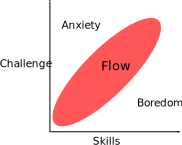
\includegraphics[width=\textwidth]{flow}
\label{fig:flow}
\caption[Short description found in the fig. table]{Long description, next to the figure}
\end{marginfigure}



\lipsum[1-3]

\begin{figure}[h!]
\begin{center}
\includegraphics[width=\textwidth]{NG2_alpha}
\end{center}
\caption[Short description found in the fig. table]{Long description, next to the figure}
\label{fig:NG_overview}
\end{figure}

\begin{figure*}[h!]
\begin{center}
\includegraphics[width=0.5\textwidth]{success}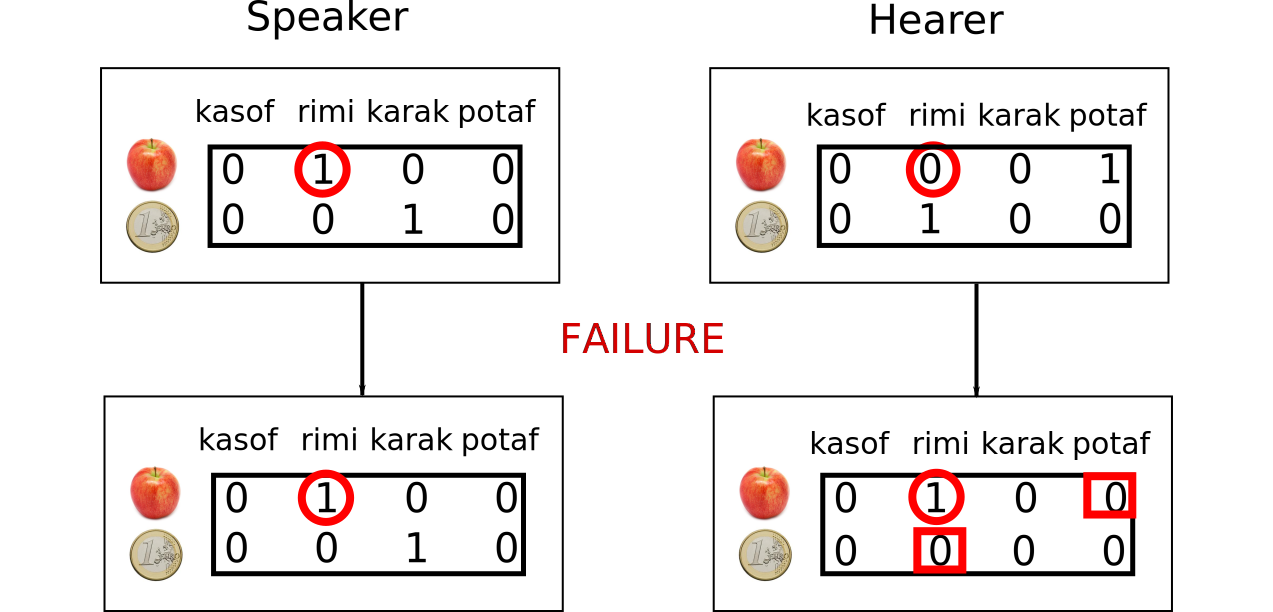
\includegraphics[width=0.5\textwidth]{fail}
\end{center}
\caption[Short description found in the fig. table]{Long description, next to the figure}
\label{fig:vocupdate}
\end{figure*}


\section{This thesis}

\subsection{Overview and structure}

This thesis introduces that, does this, and is awesome because blah. (Two general sentences to describe the work; then the content of each chapter can be described independently)

Chapter \ref{chap:chap1_fake} is a completely fake chapter with only a lorem ipsum.

Chapter \ref{chap:chap2_fake} is just the same.

\subsection{Contributions}

\begin{description}

\item[Contribution1:] \lipsum[1]

\item[Contribution2:] \lipsum[1]

\item[Contribution3:] \lipsum[1]


\end{description}

\subsection{Publications}

\begin{itemize}
\item \fullcite{schueller2015active}
\item \fullcite{schueller2016active}
\item \fullcite{schueller2018complexity}
\end{itemize}



\section{Short summary}

\lipsum[1-5]
